% !TeX encoding = UTF-8

\documentclass{protokol}

\usepackage{tikz}
\usetikzlibrary{calc}
\usetikzlibrary{arrows}

%====== Units =====
\usepackage{siunitx}
\sisetup{inter-unit-product =\ensuremath{\cdot}}
\sisetup{group-digits = integer}
\sisetup{output-decimal-marker = {,}}
\sisetup{exponent-product = \ensuremath{\cdot}}
\sisetup{separate-uncertainty}
\sisetup{tight-spacing = false}
%\sisetup{scientific-notation = true}
%\sisetup{round-mode=places,round-precision=4}
%\sisetup{evaluate-expression}


%====== Grafy =====
\usepackage{pgfplots}
\pgfplotsset{width=0.8\linewidth, compat=1.17}
\def\plotcscale{0.8}
\usepackage{pgfplotstable}
\usepackage[figurename=Graf]{caption} % figure caption rename
%====== Rovnice align block ======
\usepackage{amsmath}
\setlength{\jot}{10pt} % rozestup mezi řádky

\graphicspath{ {./img/} }

%====== Vyplňte údaje ======
\jmeno{Jakub Charvot}
\kod{240844}
\rocnik{2.}
\obor{MET}
\skupina{MET/4}
\spolupracoval{Radek Kučera}

\merenodne{10.\,11.\,2022}
\odevzdanodne{24.\,11.\,2022}
\nazev{Operační usměrňovače}
\cislo{4} %měřené úlohy

\predmet{Analogové elektronické obvody}
\ustav{Ústav mikroelektroniky}
\skola{FEKT VUT v Brně}

\def\para{x+0}
\def\parb{\para-80}

% CSV
\usepackage{blindtext}

\usepackage{subfiles} % Best loaded last in the preamble
\usepackage{datatool}

\DTLloaddb[omitlines=1]{data}{data/data.csv}
% \DTLloaddb[omitlines=2]{druha}{data/druha-cast.csv}



\begin{document}
%====== Vygenerování tabulky ======
%	\maketitle
%====== Úvodní texty protokolu ======

%	\section{Teoretický úvod}
%		\begin{figure}[h!]
    \centering
    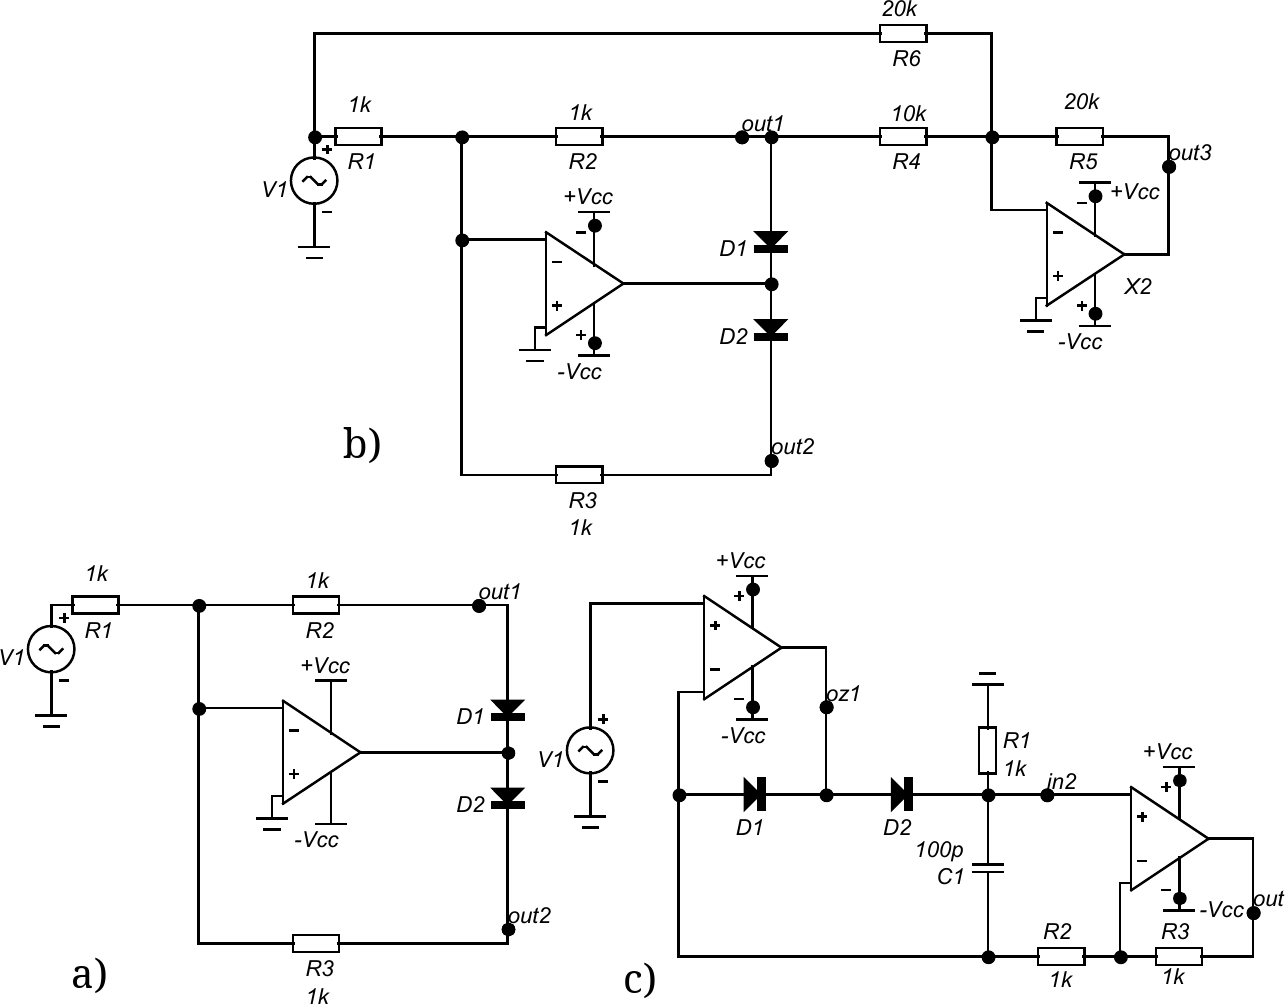
\includegraphics[width=\textwidth]{schema.png}
    \centering
    \caption{Schémata zapojení -- a) jednocestný usměrňovač, b) dvoucestný usměrňovač, c) dvoucestný usměrňovač s minimem přesných součástek.}
    \label{fig:schema}
\end{figure}



\subsection{Funkce jednotlivých zapojení}

    Operační zesilovač s OZ má za úkol překonat nedostatky, které má zapojení pouze s diodami, které díky svému prahovému napětí nedokáží usměrňovat velmi malá napětí. 
    
    Zapojení 1a) je jednocestný usměrňovač, kdy je vždy přes jednu diodu uzavřená záporná zpětná vazba a druhá dioda je uzavřená. Na výstupu je pak signál jednocestně usměrněný a invertovaný. 
    
    Zapojení 1b) pak tento signál zdvojnásobí a sečte s původním vstupním signálem, ve výsledku tedy původní záporné půlvlny zůstanou a kladné po sečtení odpovídají opět záporným. Výsledkem je tedy dvoucestně usměrněný invertovaný signál. 
    Nevýhodou tohoto zapojení je nutnost použít dva co nejshodnější odpory a k nim jeden, který odpovídá hodnotu přesně polovině, při nedodržení nebudou na výstupu půlvlny stejně velké, toto značně zdražuje zapojení. 

    Tento problém se snaží řešit zapojení 1c), kdy pro správnou funkci stačí jedna dvojice přesných odporů \( R_2\) a \(R_3\). Záporná zpětná vazba prvního OZ je vždy uzavřena přes druhý OZ, díky diodám je ale cesta zpětné vazby jiná pro kladný a pro záporný signál, takže ve výsledku je na výstupu druhého OZ signál vždy kladný, neboli dvoucestně usměrněný.   
%		
%	% \newpage
%	\section{Výsledky počítačové simulace}
%		\begin{figure}[h!]
    \centering
    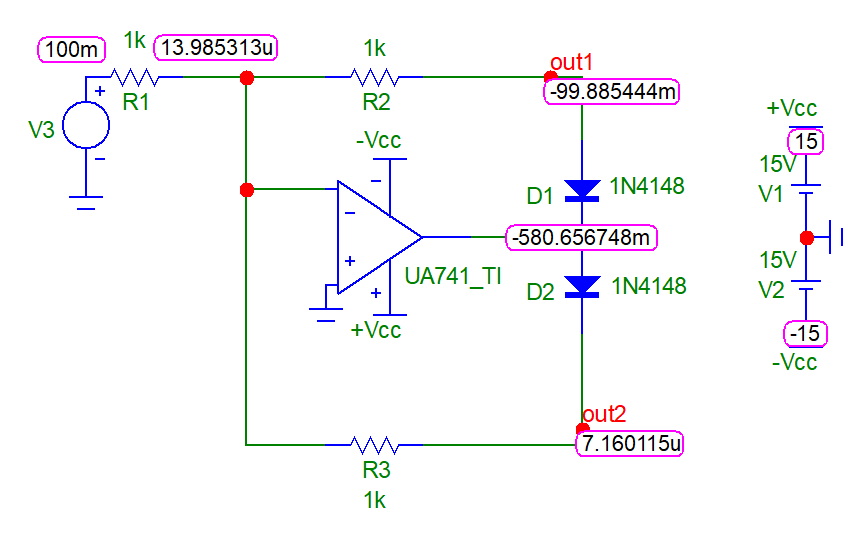
\includegraphics[width=0.63\textwidth]{microcap/1-dcbod.png}
    \caption{Zapojení a) -- stejnosměrný prac. bod pro kladné vstupní napětí.}
    \label{fig:microcap/.png}
\end{figure}

\begin{figure}[h!]
    \centering
    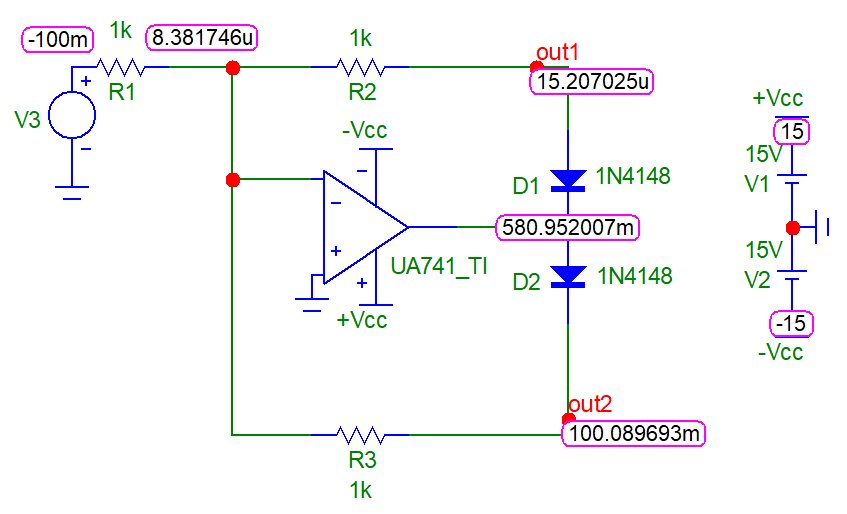
\includegraphics[width=0.63\textwidth]{microcap/1-dcbod2.png}
    \caption{Zapojení a) -- stejnosměrný prac. bod pro záporné vstupní napětí.}
    \label{fig:microcap/.png}
\end{figure}

\begin{figure}[h!]
    \centering
    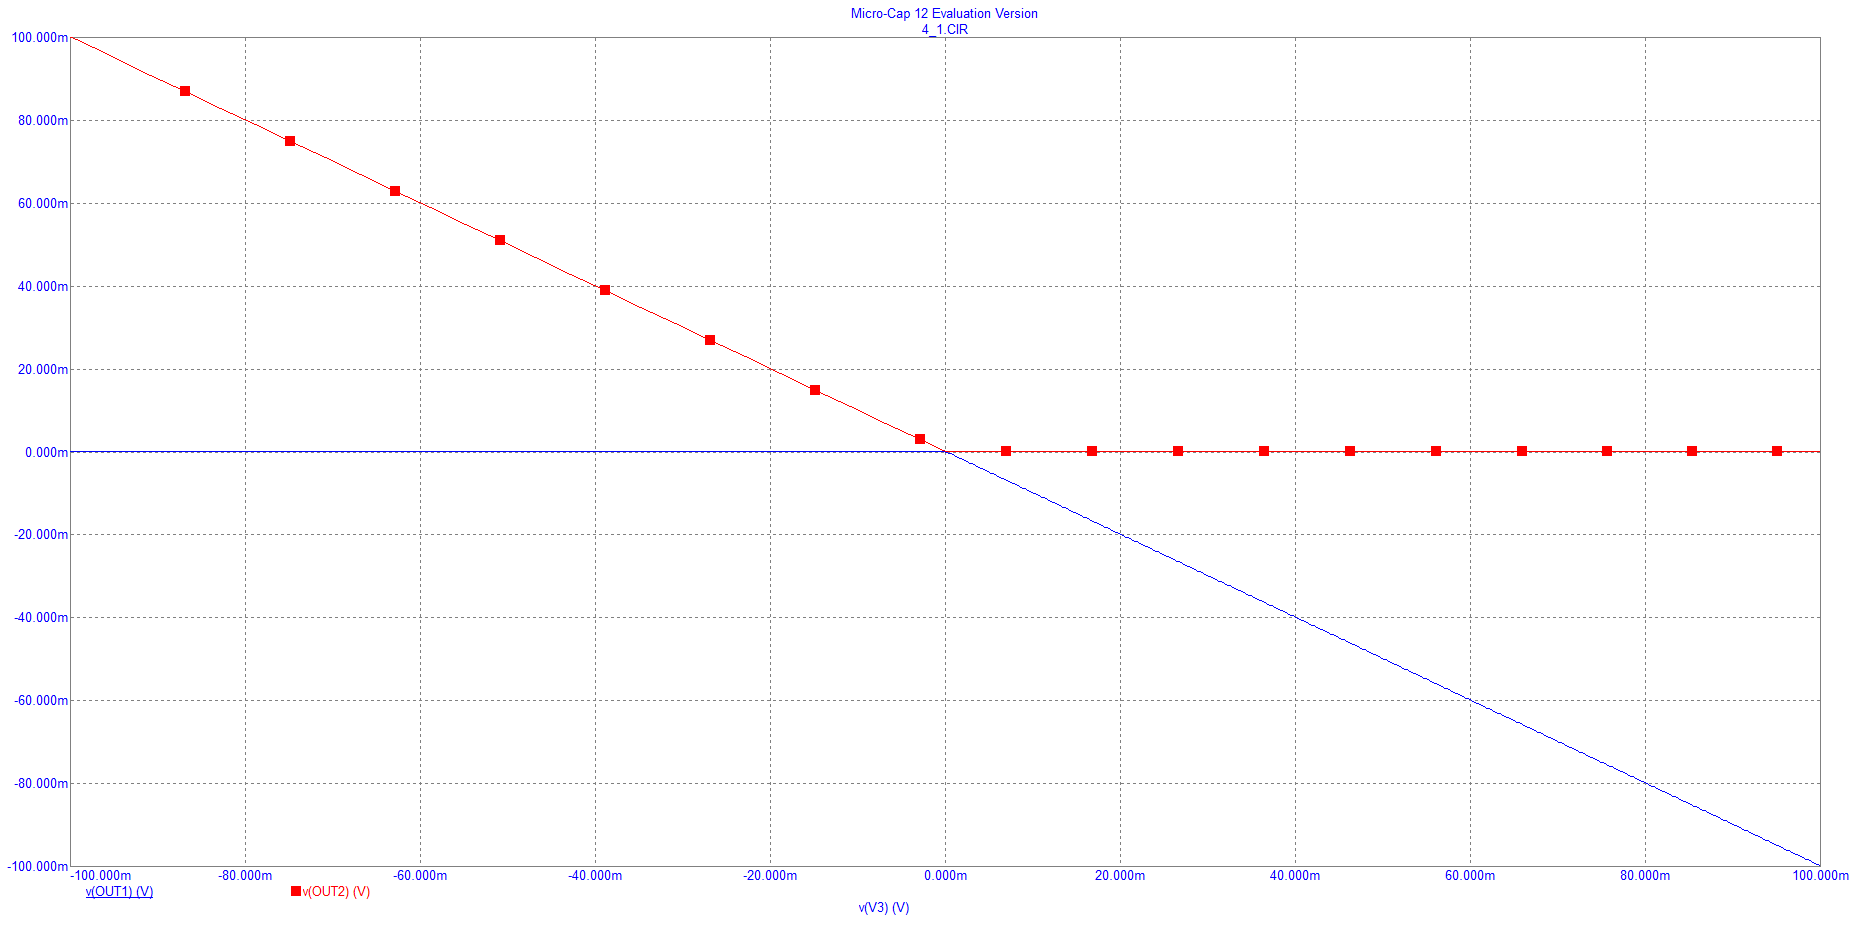
\includegraphics[width=0.8\textwidth]{microcap/1-dcprevodni.png}
    \caption{Zapojení a) -- stejnosměrná převodní charakteristika.}
    \label{fig:microcap/.png}
\end{figure}

\begin{figure}[h!]
    \centering
    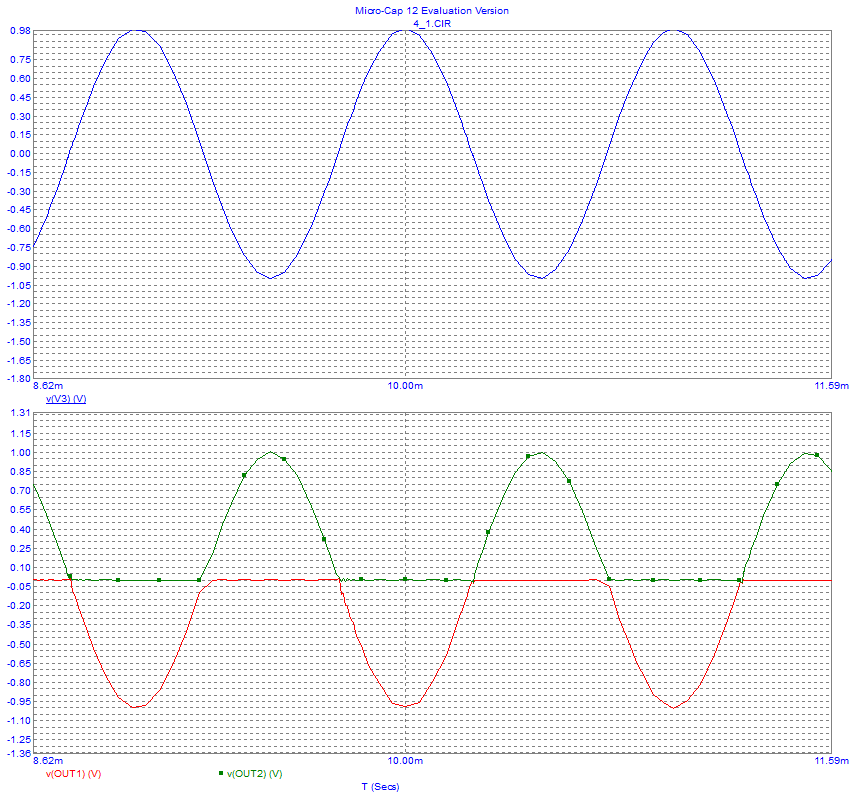
\includegraphics[width=0.8\textwidth]{microcap/1-transient-1khz-1v.png}
    \caption{Zapojení a) -- časová závislost obou výstupních napětí na vstupním napětí, jednocestné zesílení, \(f=\qty{1}{\kilo\hertz}, U_M=\qty{1}{\volt}\).}
    \label{fig:microcap/.png}
\end{figure}

\begin{figure}[h!]
    \centering
    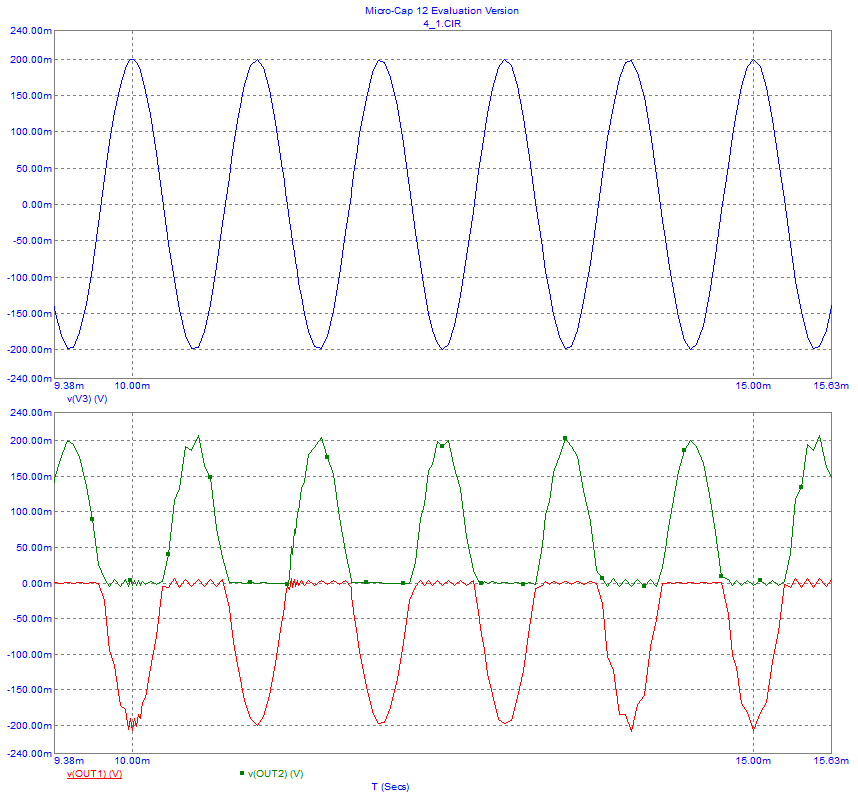
\includegraphics[width=0.7\textwidth]{microcap/1-transient-1khz-0.2v.png}
    \caption{Zapojení a) -- časová závislost obou výstupních napětí na vstupním napětí, nejmenší amplituda, při které zapojení obstojně usměrňuje, \(f=\qty{1}{\kilo\hertz}, U_M=\qty{200}{\milli\volt}\).}
    \label{fig:microcap/.png}
\end{figure}

\begin{figure}[h!]
    \centering
    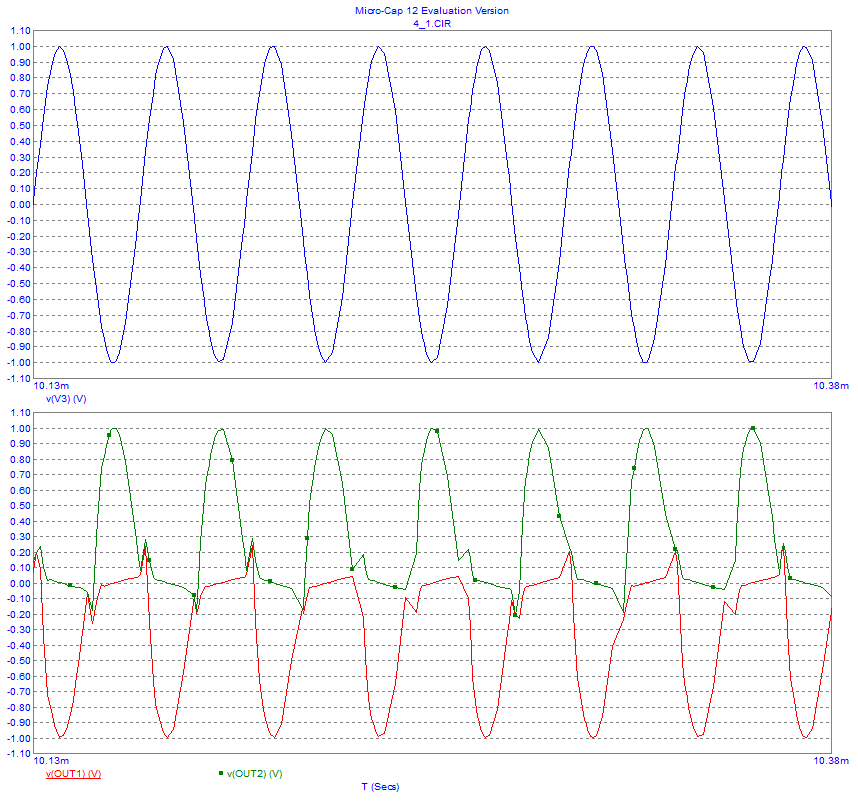
\includegraphics[width=0.7\textwidth]{microcap/1-transient-30khz-1v.png}
    \caption{Zapojení a) -- časová závislost obou výstupních napětí na vstupním napětí, nejvyšší frekvence, při které zapojení obstojně usměrňuje, \(f=\qty{30}{\kilo\hertz}, U_M=\qty{1}{\volt}\).}
    \label{fig:microcap/.png}
\end{figure}

\begin{figure}[h!]
    \centering
    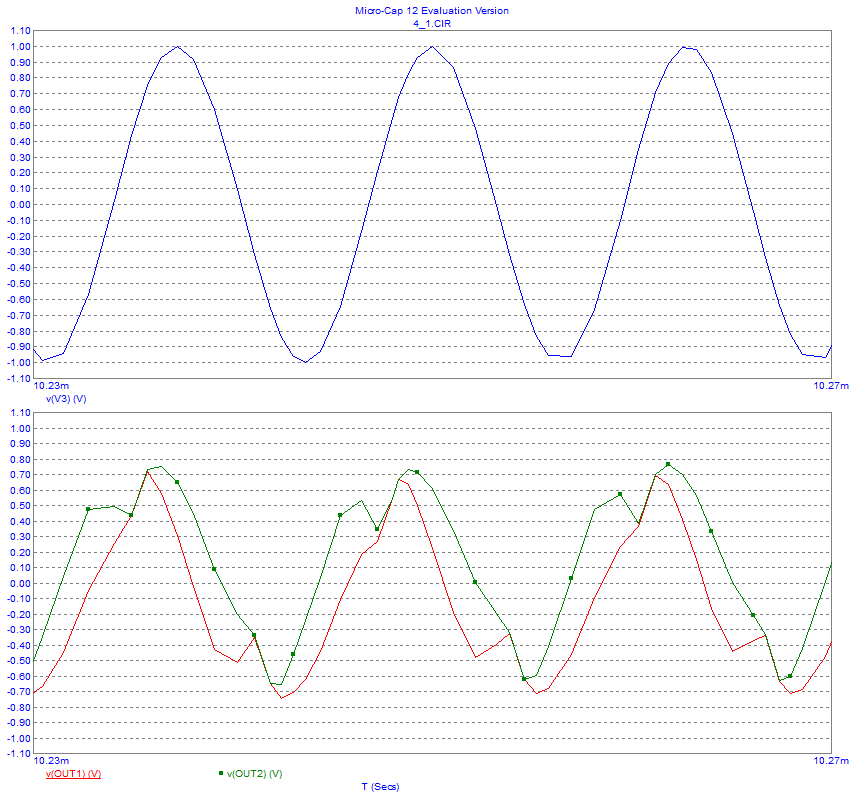
\includegraphics[width=0.8\textwidth]{microcap/1-transient-100khz-1v.png}
    \caption{Zapojení a) -- časová závislost obou výstupních napětí na vstupním napětí, příliš vysoká frekvence, k usměrnění nedochází vůbec, \(f=\qty{100}{\kilo\hertz}, U_M=\qty{1}{\volt}\).}
    \label{fig:microcap/.png}
\end{figure}    

% \begin{figure}[h!]
%     \centering
%     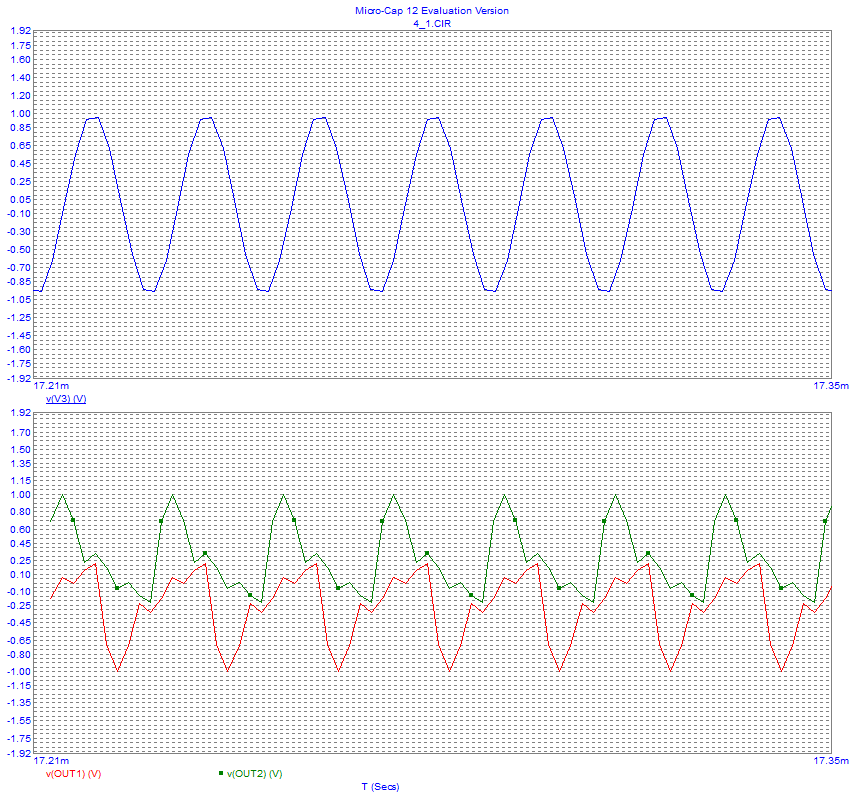
\includegraphics[width=0.8\textwidth]{microcap/1-transient-50khz-1v.png}
%     \caption{microcap/.png}
%     \label{fig:microcap/.png}
% \end{figure}

\begin{figure}[h!]
    \centering
    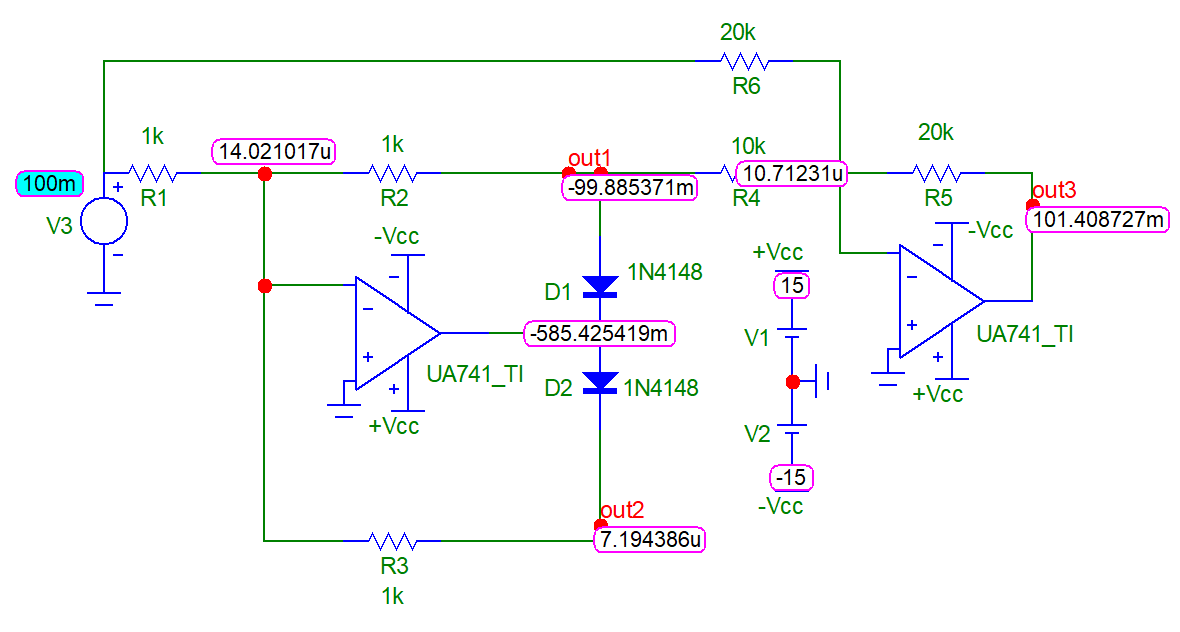
\includegraphics[width=0.8\textwidth]{microcap/2-dcbod.png}
    \caption{Zapojení b) -- stejnosměrný prac. bod při kladném napětí na vstupu, na výstupu kladné napětí.}
    \label{fig:microcap/.png}
\end{figure}

\begin{figure}[h!]
    \centering
    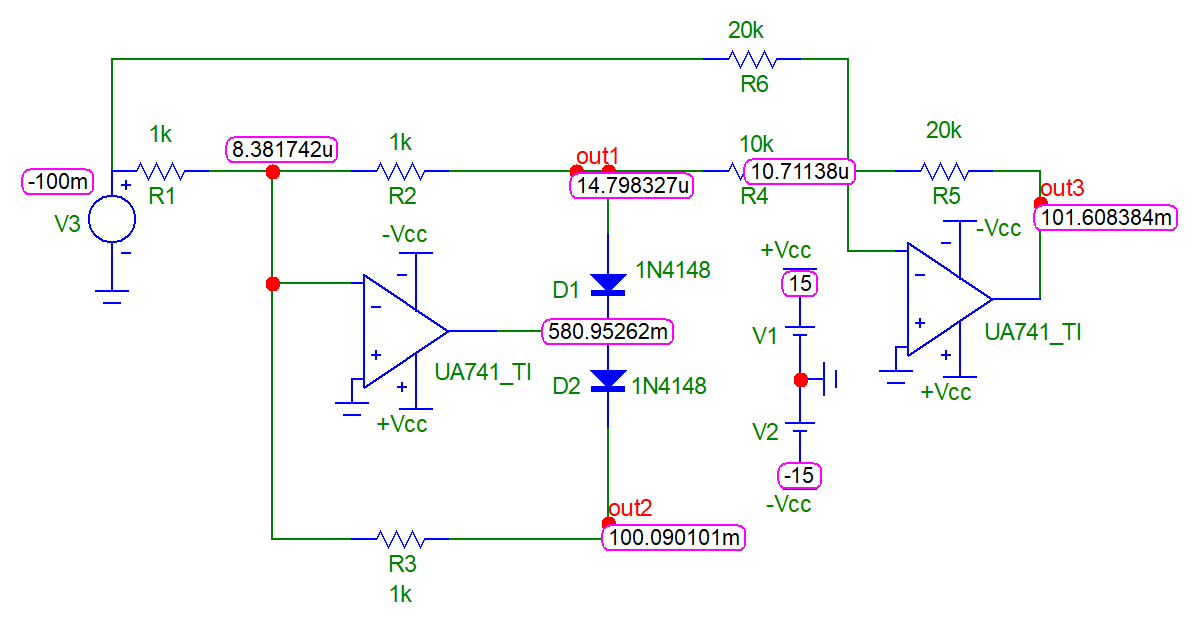
\includegraphics[width=0.61\textwidth]{microcap/2-dcbod2.png}
    \caption{Zapojení b) -- stejnosměrný prac. bod při záporném napětí na vstupu, na výstupu opět kladné napětí.}
    \label{fig:microcap/.png}
\end{figure}

\begin{figure}[h!]
    \centering
    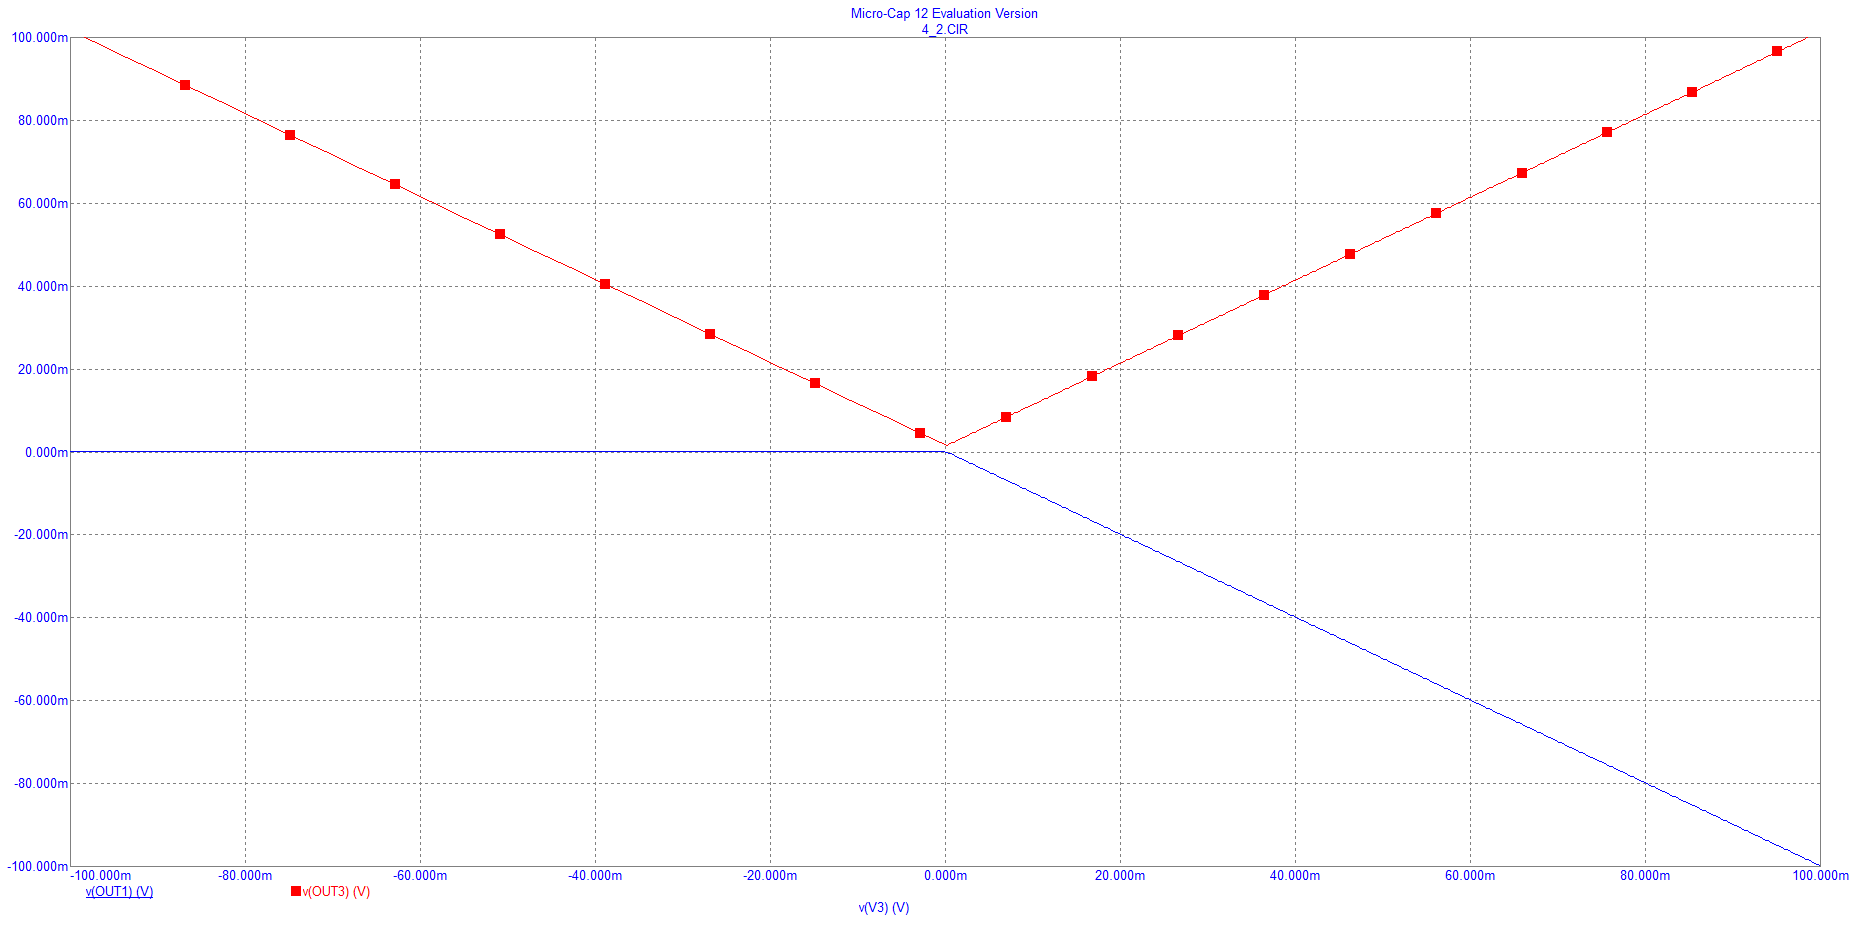
\includegraphics[width=0.61\textwidth]{microcap/2-dcprevodni.png}
    \caption{Zapojení b) -- stejnosměrná převodní charakteristika dvoucestného usměrnění.}
    \label{fig:microcap/.png}
\end{figure}

\begin{figure}[h!]
    \centering
    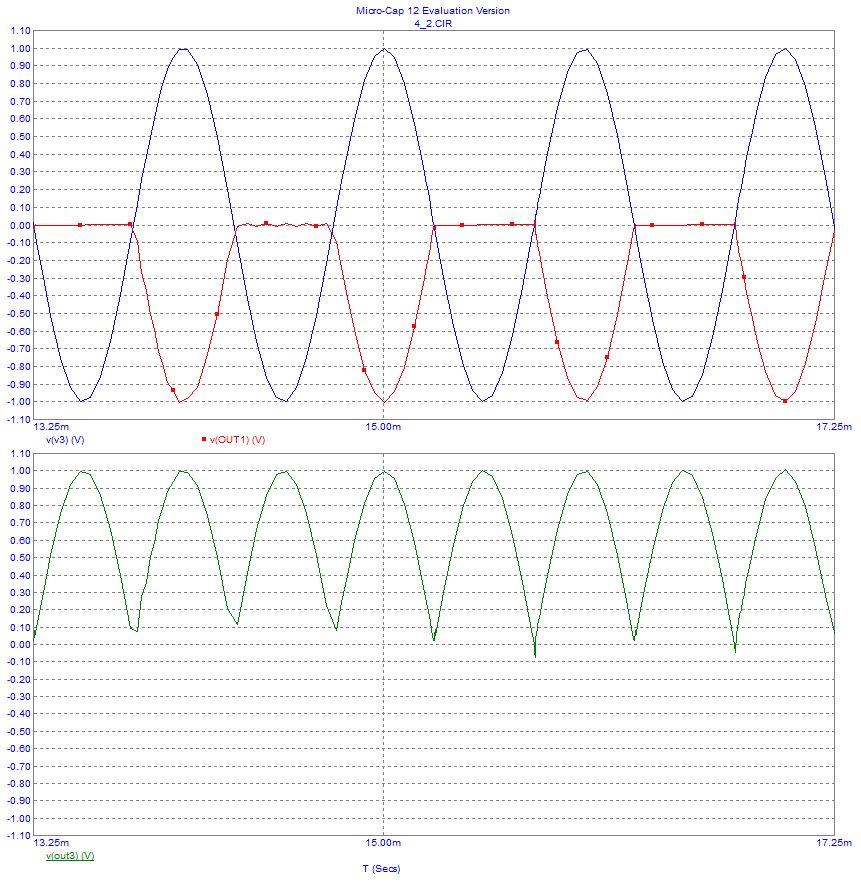
\includegraphics[width=0.61\textwidth]{microcap/2-transient-1khz-1v.png}
    \caption{Zapojení b) -- časová závislost napětí na výstupech obou OZ na vstupním napětí, jednocestné a dvoucestné usměrnění, \(f=\qty{1}{\kilo\hertz}, U_M=\qty{1}{\volt}\).}
    \label{fig:microcap/.png}
\end{figure}

% \begin{figure}[h!]
%     \centering
%     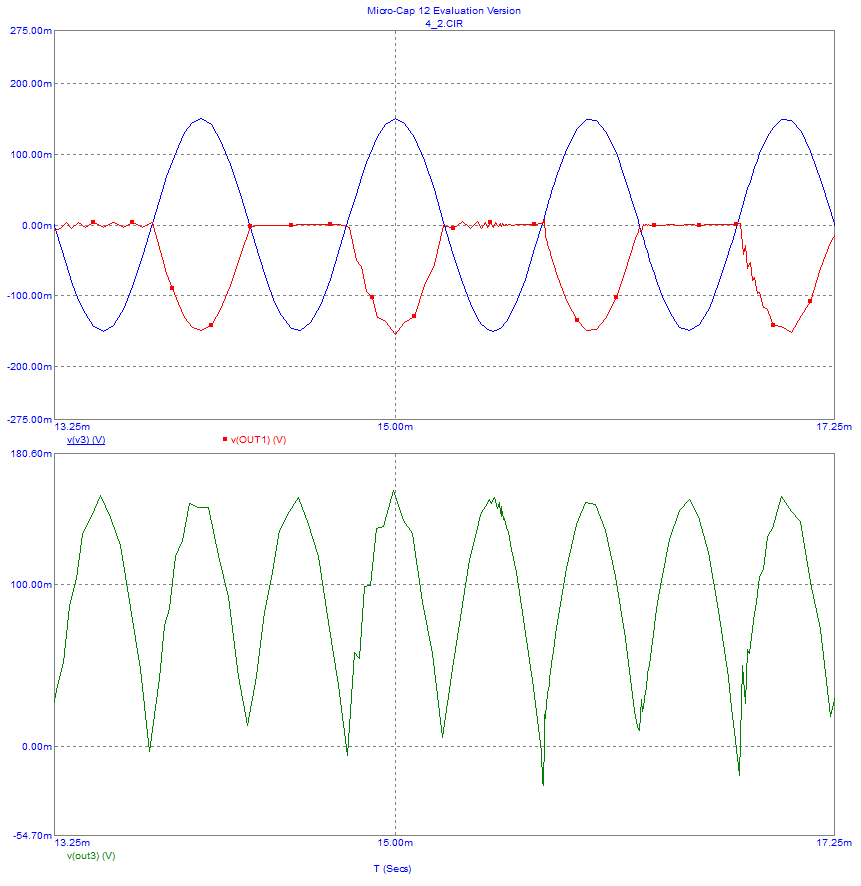
\includegraphics[width=0.8\textwidth]{microcap/2-transient-1khz-0.15v.png}
%     \caption{Zapojení b) -- časová závislost napětí na výstupech obou OZ na vstupním napětí, nejmenší amplituda, při které uspokojivě usměrňuje, \(f=\qty{1}{\kilo\hertz}, U_M=\qty{150}{\milli\volt}\).}
%     \label{fig:microcap/.png}
% \end{figure}

\begin{figure}[h!]
    \centering
    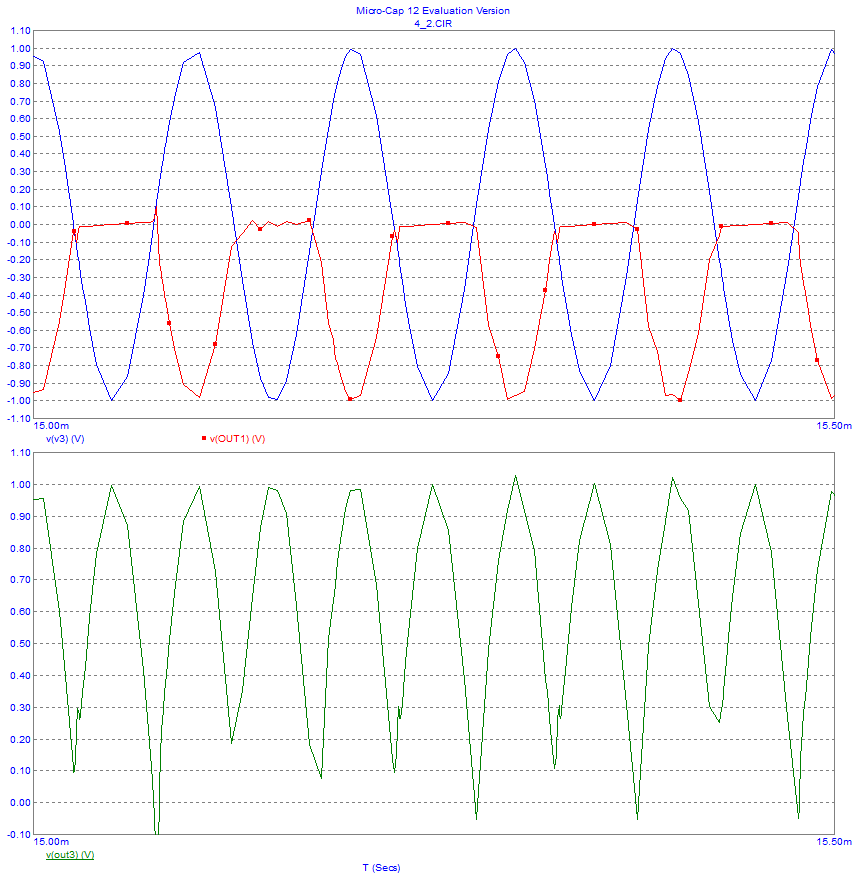
\includegraphics[width=0.7\textwidth]{microcap/2-transient-10khz-1v.png}
    \caption{Zapojení b) -- časová závislost napětí na výstupech obou OZ na vstupním napětí, nejvyšší frekvence, při které uspokojivě usměrňuje, \(f=\qty{10}{\kilo\hertz}, U_M=\qty{1}{\volt}\).}
    \label{fig:microcap/.png}
\end{figure}

\begin{figure}[h!]
    \centering
    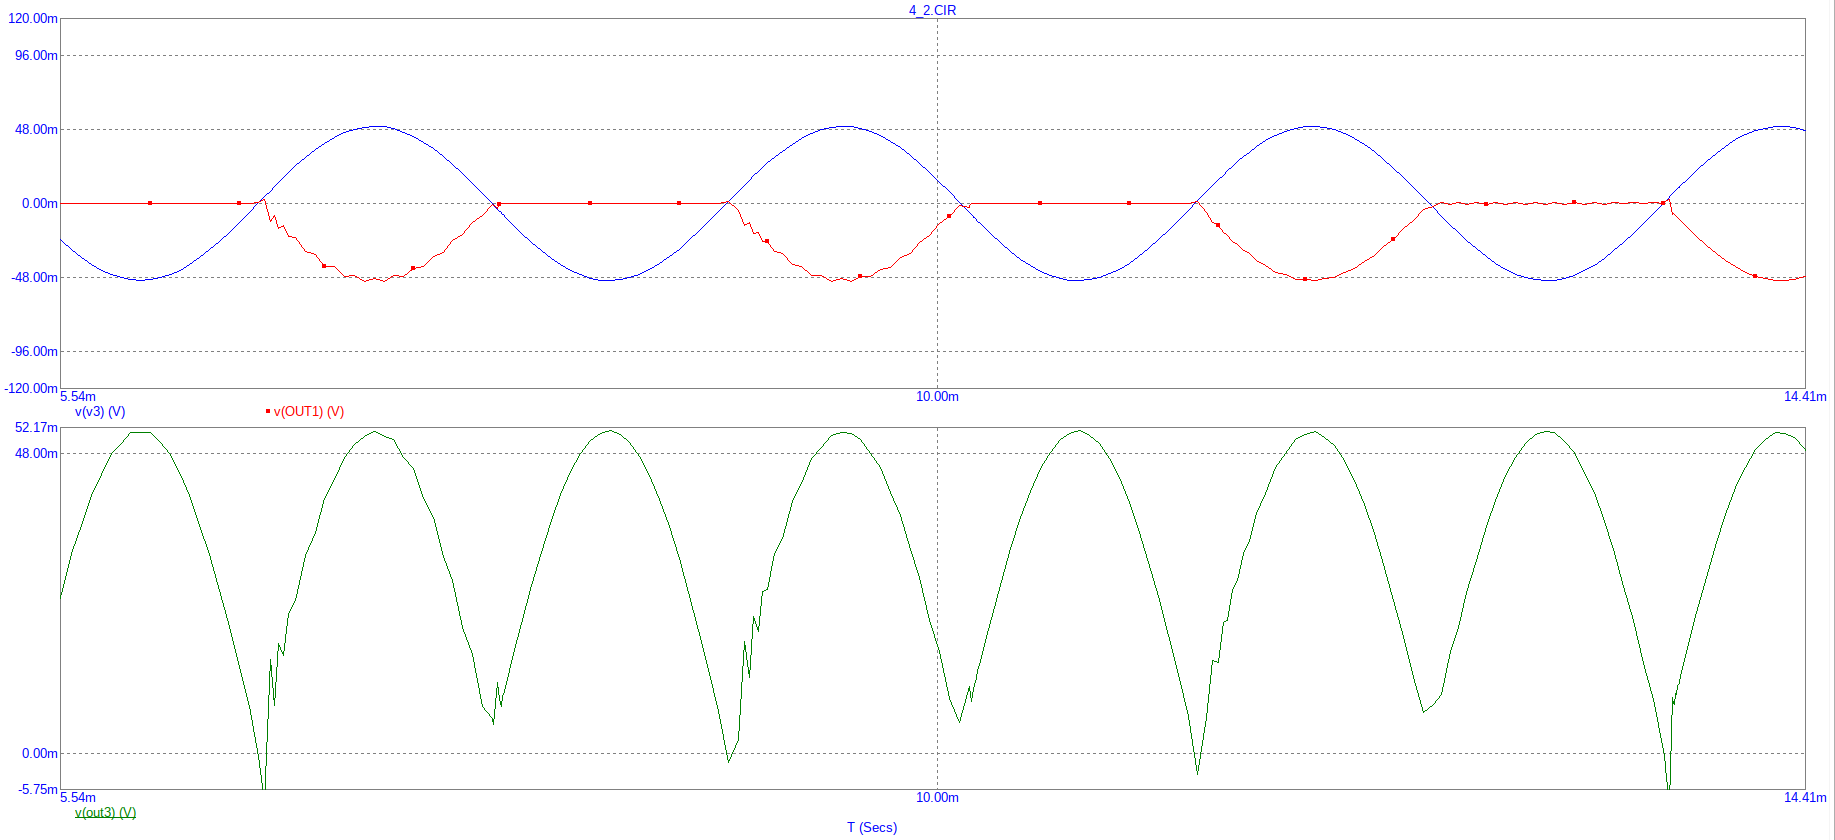
\includegraphics[width=0.7\textwidth]{microcap/2-transient-420hz-0.05v.png}
    \caption{Zapojení b) -- časová závislost napětí na výstupech obou OZ na vstupním napětí, nejnižší amplituda, při které uspokojivě usměrňuje, \(f=\qty{420}{\hertz}, U_M=\qty{50}{\milli\volt}\).}
    \label{fig:microcap/.png}
\end{figure}

\begin{figure}[h!]
    \centering
    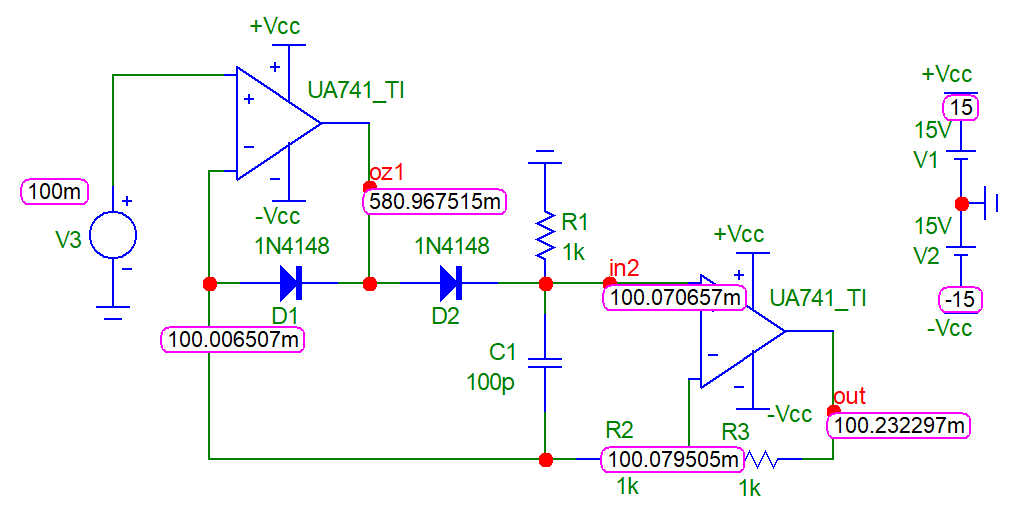
\includegraphics[width=0.8\textwidth]{microcap/3-dcbod.png}
    \caption{Zapojení c) -- stejnosměrný prac. bod při kladném napětí na vstupu, na výstupu kladné napětí.}
    \label{fig:microcap/.png}
\end{figure}

\begin{figure}[h!]
    \centering
    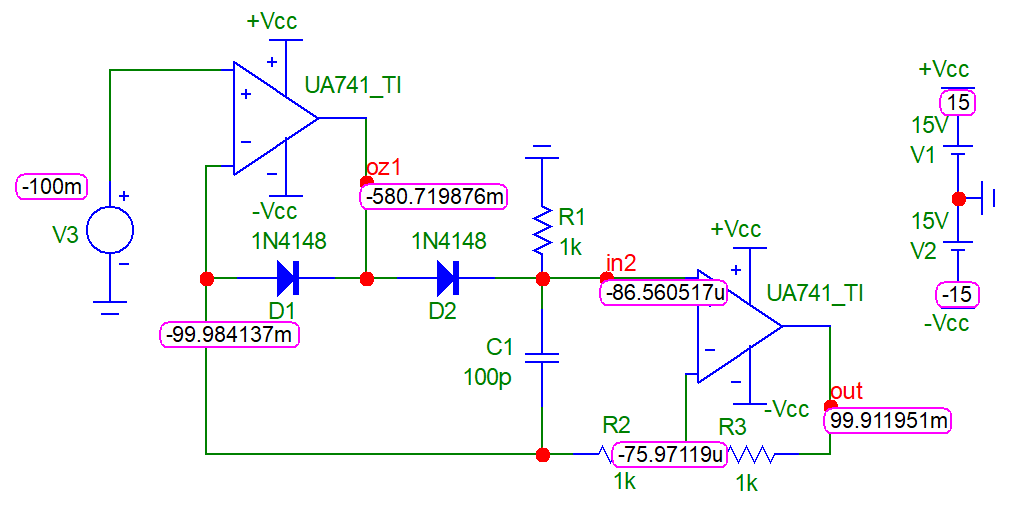
\includegraphics[width=0.8\textwidth]{microcap/3-dcbod2.png}
    \caption{Zapojení c) -- stejnosměrný prac. bod při záporném napětí na vstupu, na výstupu kladné napětí.}
    \label{fig:microcap/.png}
\end{figure}

\begin{figure}[h!]
    \centering
    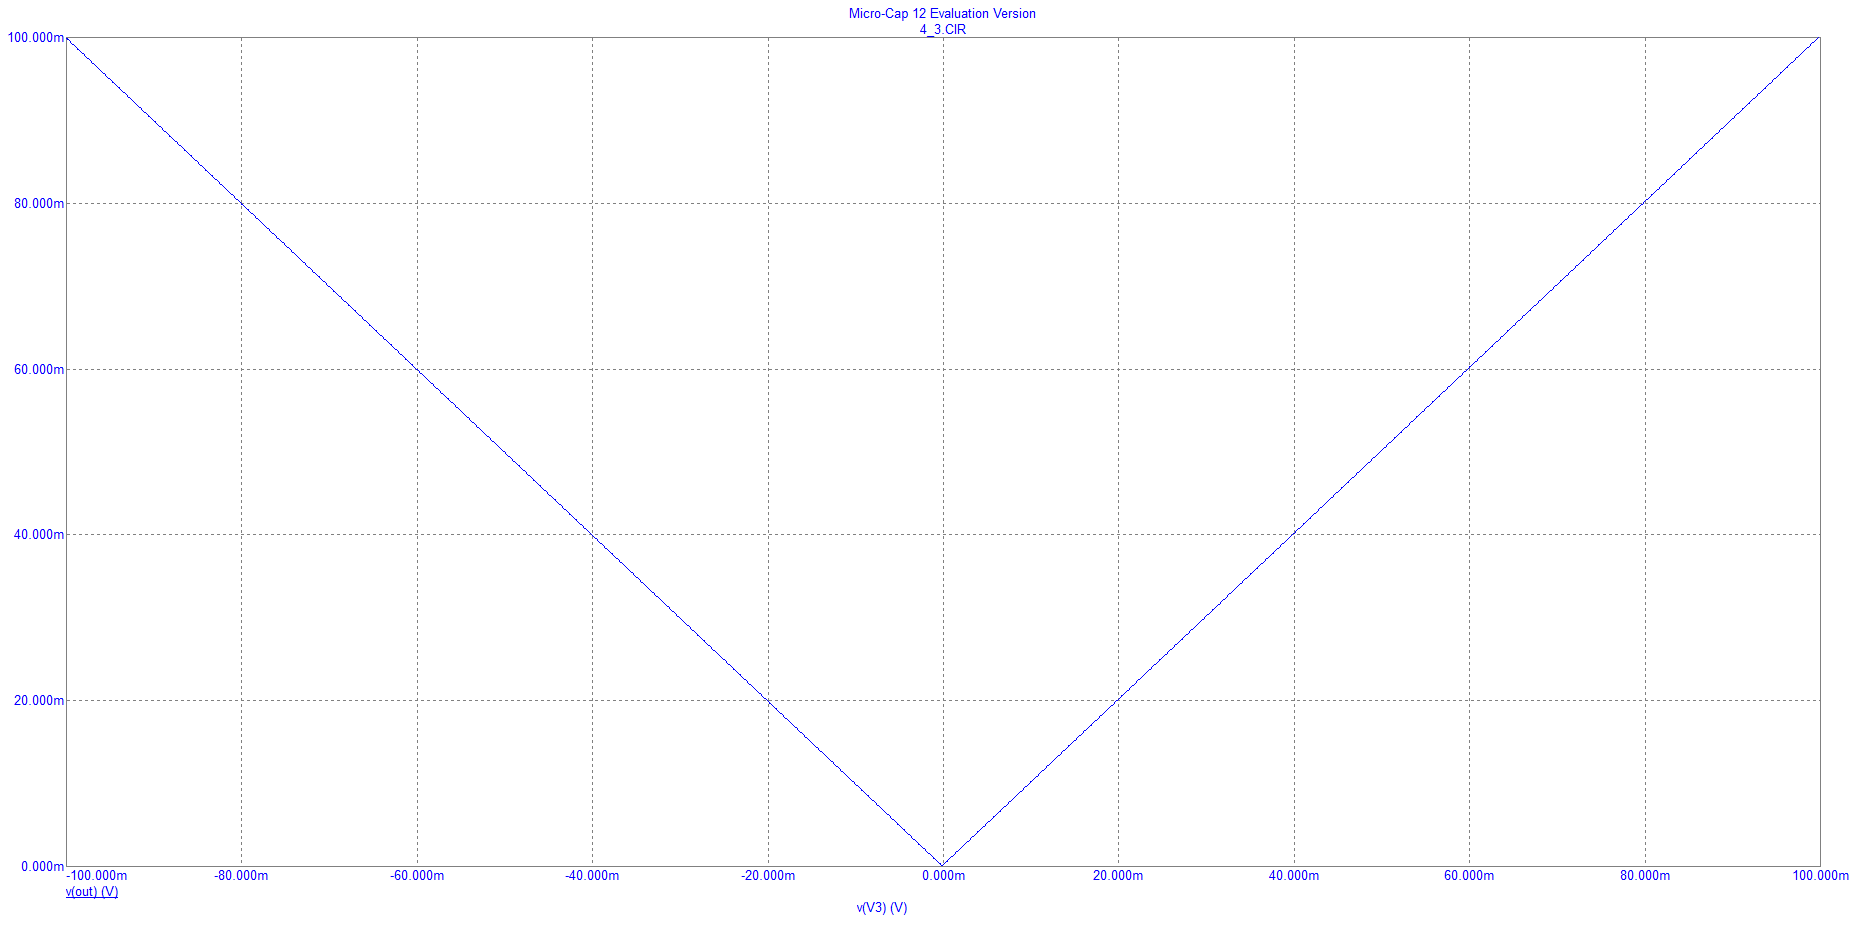
\includegraphics[width=0.8\textwidth]{microcap/3-dcprevodni.png}
    \caption{Zapojení c) -- stejnosměrná převodní charakteristika.}
    \label{fig:microcap/.png}
\end{figure}

\begin{figure}[h!]
    \centering
    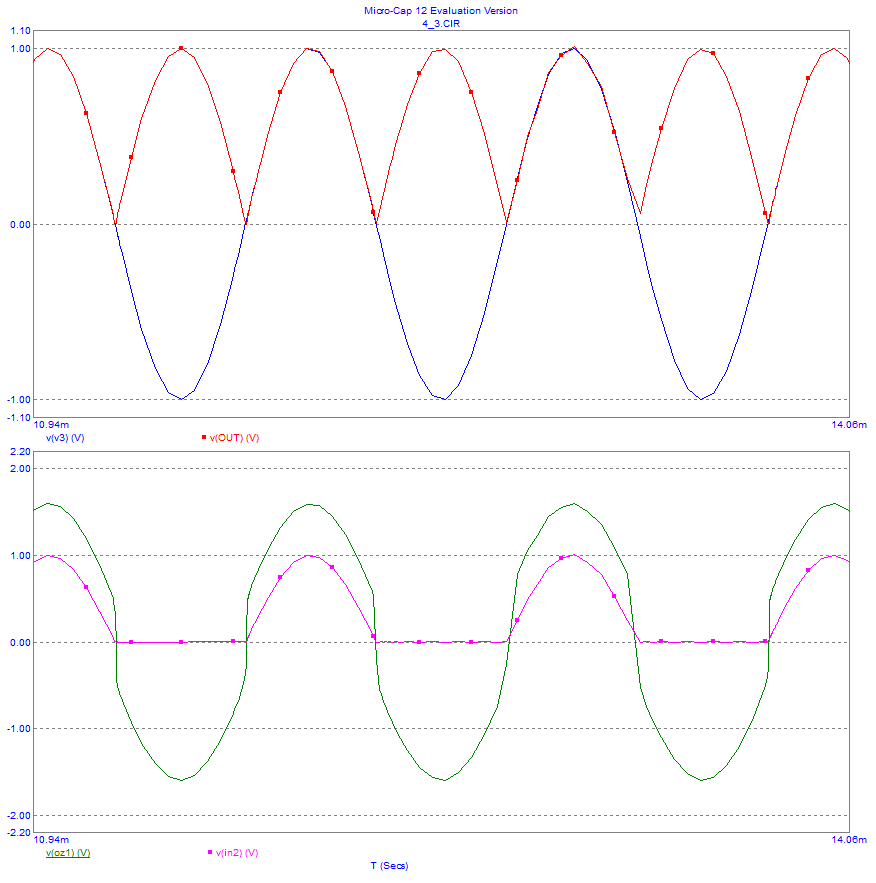
\includegraphics[width=0.66\textwidth]{microcap/3-transient-1khz-1v.png}
    \caption{Zapojení c) -- časová závislost napětí na výstupech obou OZ na vstupním napětí, jednocestné a dvoucestné usměrnění, \(f=\qty{1}{\kilo\hertz}, U_M=\qty{1}{\volt}\).}
    \label{fig:microcap/.png}
\end{figure}

\begin{figure}[h!]
    \centering
    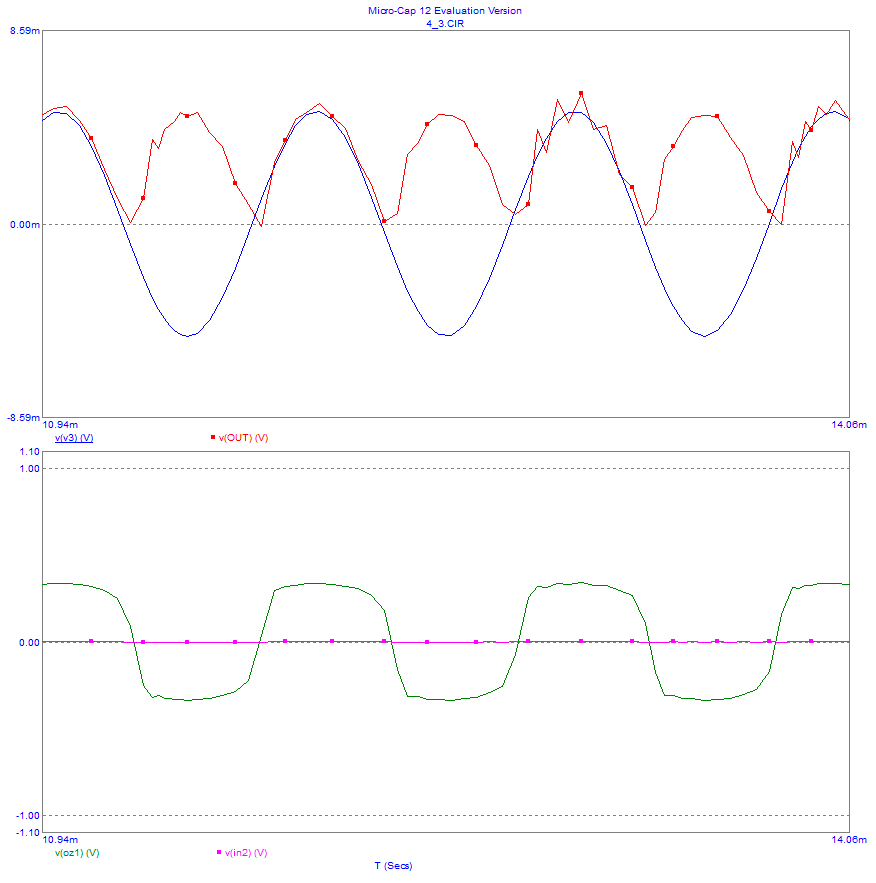
\includegraphics[width=0.66\textwidth]{microcap/3-transient-1khz-5mv.png}
    \caption{Zapojení c) -- časová závislost napětí na výstupech obou OZ na vstupním napětí, nejnižší amplituda, při které uspokojivě usměrňuje, \(f=\qty{1}{\kilo\hertz}, U_M=\qty{5}{\milli\volt}\).}
    \label{fig:microcap/.png}
\end{figure}

% \begin{figure}[h!]
%     \centering
%     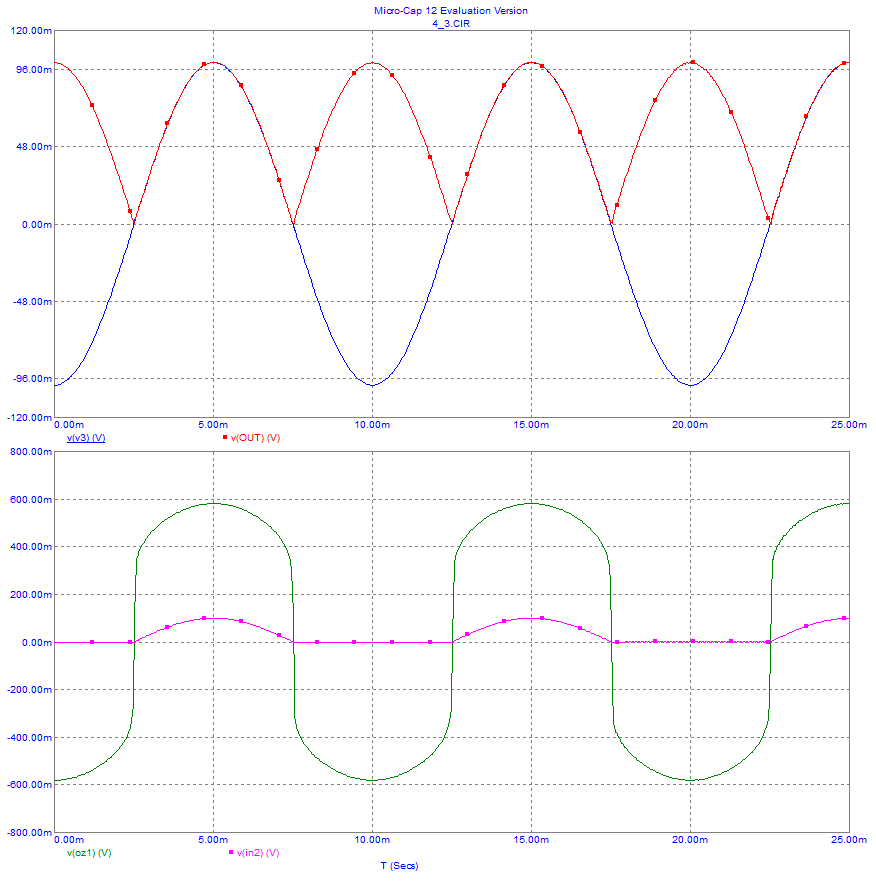
\includegraphics[width=0.8\textwidth]{microcap/3-transient-100hz-0.1v.png}
%     \caption{microcap/.png}
%     \label{fig:microcap/.png}
% \end{figure}

\begin{figure}[h!]
    \centering
    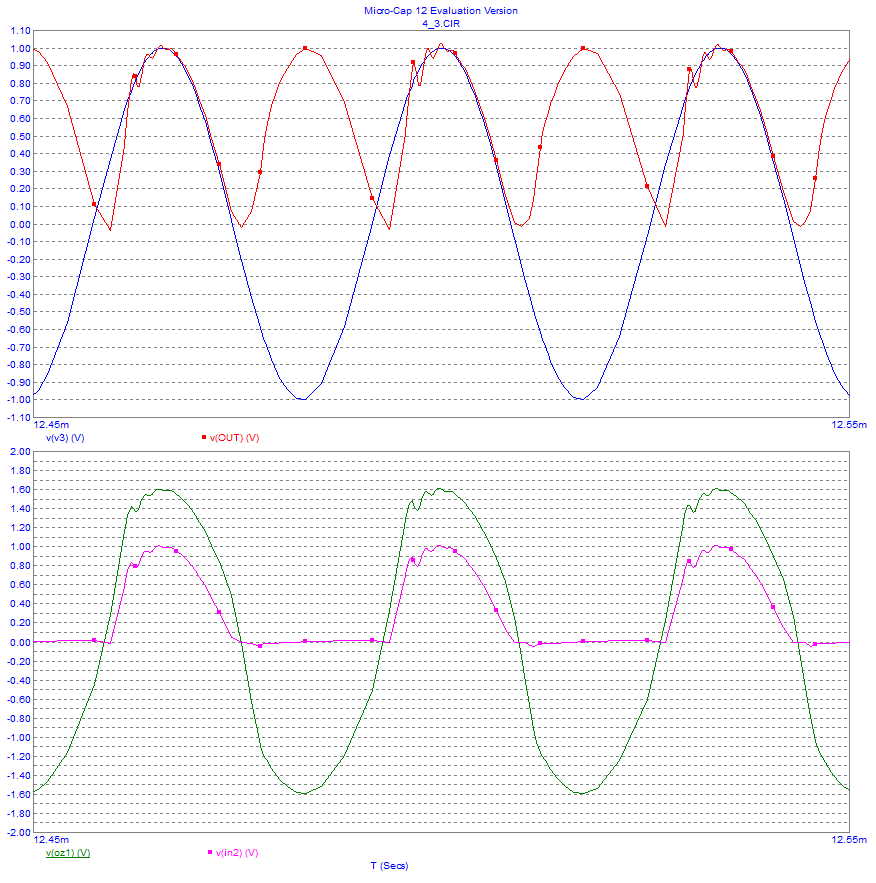
\includegraphics[width=0.8\textwidth]{microcap/3-transient-30khz-1v.png}
    \caption{Zapojení c) -- časová závislost napětí na výstupech obou OZ na vstupním napětí, nejvyšší frekvence, při které uspokojivě usměrňuje, \(f=\qty{30}{\kilo\hertz}, U_M=\qty{1}{\volt}\).}
    \label{fig:microcap/.png}
\end{figure}


%		

%	\clearpage

\section{Zpracování měřených hodnot}
	\begin{table}[h!]
		\centering
		\def\arraystretch{1.4}
		\begin{tabular}{ |l|l|l|l|l|l| }
			\hline
			Převod &
			Zátěž [\unit{\ohm}] &
			\(Q\ [\unit{\litre\per\hour}]\) &
			\(p\ [\unit{\kilo\pascal}]\) &
			\(U\ [\unit{\volt}]\) &
			\(f\ [\unit{\hertz}]\)
			%
			\DTLforeach{data}{\A=prevod,\B=R,\C=Q,\D=p,\E=U,\F=f, \G=I,\H=Pt,\I=Pg,\J=Qt,\K=etha,\L=H}
			{\DTLiffirstrow{\\ \hline \hline}{\\ \hline} %
			\A & 
			\B &
			\C &
			\D &
			\E &
			\F 
			}\\ \hline
		\end{tabular}
		\caption{Naměřené hodnoty.}
		\label{tab:tabulka-hodnot}
	\end{table}
	
	\subsection{Příklady výpočtu}
	\[
		Q_{T} = S_{2} \cdot \sqrt{{\frac{2\cdot p}{\rho_{v}  \cdot (1-{\frac{S_{2} }{S_{1}}}^2)}}}\cdot1000\cdot3600\ [\unit{\litre\per\hour}]
	\]
	
	\[
		Q_{T} = \num{4.91e-6} \cdot \sqrt{{\frac{2\cdot \num{8000}}{997  \cdot (1-{\frac{\num{4.91e-6}}{\num{2.84e-4}}}^2)}}}\cdot1000\cdot3600\ = \SI{70,8}{\litre\per\hour}
	\]
	
	\[
		P_T=0,65 \cdot g \cdot Q_M \cdot H \cdot \rho
	\]
	
	\[
		P_T=0,65 \cdot 9,81 \cdot 300 \cdot 0,818 \cdot 997 = \SI{0,4333}{\watt}
	\]
	
	\[
		P_{G} = U \cdot I 
	\]
	
	\[
		P_{G} = 2,47 \cdot 0,247 = \SI{0,6101}{\watt}
	\]

\begin{table}[h!]
	\centering
	\def\arraystretch{1.4}
	\begin{tabular}{ |l|l|l|l|l|l|l|l|l| }
		\hline
		Převod &
		Zátěž [\unit{\ohm}] &
		\(Q\ [\unit{\litre\per\hour}]\) &
		\(I\ [\unit{\ampere}]\) &
		\(P_{T}\ [\unit{\watt}]\) &
		\(P_{G} \ [\unit{\watt}]\) &
		\(\eta\ [-]\) &
		\(Q_{T} \ [\unit{\litre\per\hour}]\) &
		\(H\ [\unit{\meter}]\) 
%
		\DTLforeach{data}{\A=prevod,\B=R,\C=Q,\D=p,\E=U,\F=f, \G=I,\H=Pt,\I=Pg,\J=Qt,\K=etha,\L=H}
		{\DTLiffirstrow{\\ \hline \hline}{\\ \hline} %
			\A & 
			\B &
			\C &
			\G &
			\H &
			\I &
			\K &
			\J &
			\L 
			}\\ \hline
	\end{tabular}
	\caption{Vypočtené hodnoty.}
	\label{tab:tabulka-hodnot}
\end{table}

\begin{figure*}[h!]
	\begin{tikzpicture}
		\centering
		\begin{axis}
			[
			xlabel={Zátěž\ [\unit{\ohm}]},
			ylabel={\( P_{G} \ [\unit{\watt}]\)},
			axis y line*=left, % dve y osy
			width=1\textwidth,
			height = 0.41\textwidth,
			legend pos=south west,
%			xmin=0,
%			ymin=0,
%			xmax=100
%			ymax=100
			]

			\addplot[mark=x, mark options={solid}, thick, blue, solid, mark size=3pt] table [skip first n=1, x=R, y=Pg, col sep=comma] {data/graf.csv};
			\addlegendentry{Výkon terbíny.}
		\end{axis}   
	 
		
		% Second y axis 
		\begin{axis}
			[
			ylabel={\( \eta\ [-]\)},
			axis x line=none,
			axis y line*=right,
			width=1\textwidth,
			height = 0.41\textwidth,
			legend pos=north east,
%			xmin=0,
%			ymin=0,
%			xmax=100
%			ymax=100
			]

			\addplot[mark=+, mark options={solid}, thick, red, solid, mark size=3pt] table [skip first n=1, x=R, y=eta, col sep=comma] {data/graf.csv};
			
			\addlegendentry{Účinnost}
		
	\end{axis}

	\end{tikzpicture}
	\caption{Závislost vypočteného výkonu a účinnosti turbíny na odporu zátěže.}
\end{figure*}

\section{Závěr}
	Dle zadání a pokynů učitele jsme pečlivě změřili všechny zadané části úlohy. Z naměřených hodnot jsme na základě vztahů uvedených v zadání vypočetli odhadovaný výkon a účinnost modelu peltonovy turbíny při různých scénářích. Výsledky nás velmi překvapili, jelikož naše účinnost se pohybovala v rozmezí 15 až 215 \unit{\percent}, přičemž hodnoty vyšší než \SI{100}{\percent} nám vyšly několikrát a to vždy pro nejnižší zátěž. 
	Pokud budeme předpokládat, že jsme nevytvořili perpetum mobile 2. druhu, musíme někde v procesu měření hledat chybu. Pokud při výpočtech ovlivníme hodnoty měřených veličin v rozptylu, který by mohl způsobit nepozorný pracovník špatným odečtením hodnoty, výsledky se změní jen nepatrně, lidský faktor tedy můžeme vyloučit. Chyba tedy může být způsobena buďto špatným případně špatně nastaveným měřícím přístrojem a nebo chybnými výpočetními vztahy. Můj odhad cílí na měřič průtoku vody, hodnota 300 popř. 600 l/h se mi zdá pocitově poněkud malá na to, jak proud vody působil.  Naopak teoretické hodnoty průtoku vyšly ještě podstatně nižší, takže bez dalšího měření není možné tento odhad potvrdit.
	Vzhledem k nepřesnosti vypočtených hodnot jsou jakékoliv další vyvozené závěry neprůkazné a zatížené hrubou chybou.


\end{document}